\section{Câu hỏi 1: Xu hướng, mùa vụ và cấu trúc tự tương quan}
\label{sec:q1}

\subsection{Phân bố và mức nền của chuỗi}

Trong toàn bộ giai đoạn, lưu lượng trung bình là \QMean{} m\textsuperscript{3}/s,
trung vị là \QMedian{} m\textsuperscript{3}/s, độ lệch chuẩn mẫu là \QStd{}
m\textsuperscript{3}/s. Giá trị nhỏ nhất là \QMin{} m\textsuperscript{3}/s và lớn
nhất là \QMax{} m\textsuperscript{3}/s. Trung vị lớn hơn trung bình cho thấy phân bố
có đuôi thấp dài: phần lớn ngày nằm ở mức trung bình đến cao, nhưng một số giai đoạn
lưu lượng rất thấp kéo trung bình xuống. Đây là đặc điểm thường gặp khi chuỗi có
nhiều năm hạn hán hoặc khi mức nền thay đổi theo thời kỳ.

Phân bố theo tháng được trình bày trong Bảng~\ref{tab:monthly-stats}. Trung bình
tháng thấp nhất là \MonthlyMinValue{} m\textsuperscript{3}/s vào tháng
\MonthlyMinMonth{}, cao nhất là \MonthlyMaxValue{} m\textsuperscript{3}/s vào tháng
\MonthlyMaxMonth{}. Chênh lệch trung bình giữa tháng cao nhất và thấp nhất chỉ khoảng
\MonthlyAmplitude{} m\textsuperscript{3}/s, tức chưa đến 3\% của mức trung bình toàn
chuỗi. Tuy nhiên, độ lệch chuẩn trong từng tháng rất lớn, dao động từ 91,79 đến
107,35 m\textsuperscript{3}/s. Nói cách khác, sự khác biệt giữa các ngày trong cùng
một tháng lớn hơn nhiều so với sự khác biệt giữa trung bình các tháng.

\begin{table}[H]
\centering
\footnotesize
\setlength{\tabcolsep}{3.2pt}
\begin{tabular}{lrrrrrrrr}
\toprule
Tháng & n & Mean & Median & SD & Min & P25 & P75 & Max \\
\midrule
T1 & 434 & 293{,}44 & 327{,}00 & 99{,}63 & 94{,}39 & 238{,}34 & 371{,}75 & 423{,}21 \\
T2 & 395 & 296{,}80 & 342{,}35 & 106{,}30 & 102{,}33 & 216{,}08 & 381{,}00 & 446{,}39 \\
T3 & 434 & 296{,}95 & 338{,}34 & 107{,}35 & 106{,}91 & 198{,}14 & 379{,}49 & 457{,}49 \\
T4 & 420 & 293{,}31 & 339{,}97 & 104{,}20 & 103{,}28 & 194{,}20 & 379{,}13 & 433{,}06 \\
T5 & 434 & 293{,}59 & 336{,}36 & 103{,}35 & 104{,}30 & 199{,}70 & 387{,}78 & 424{,}66 \\
T6 & 420 & 296{,}18 & 332{,}75 & 104{,}06 & 105{,}84 & 192{,}71 & 386{,}04 & 443{,}99 \\
T7 & 434 & 296{,}25 & 328{,}04 & 100{,}32 & 111{,}16 & 208{,}79 & 378{,}20 & 453{,}52 \\
T8 & 434 & 294{,}69 & 315{,}12 & 93{,}87 & 111{,}01 & 214{,}25 & 369{,}49 & 449{,}08 \\
T9 & 420 & 292{,}32 & 315{,}45 & 92{,}23 & 120{,}18 & 215{,}86 & 370{,}45 & 429{,}67 \\
T10 & 434 & 294{,}55 & 311{,}10 & 94{,}79 & 121{,}19 & 226{,}93 & 377{,}89 & 439{,}97 \\
T11 & 420 & 300{,}16 & 324{,}61 & 93{,}52 & 114{,}17 & 230{,}98 & 384{,}04 & 428{,}14 \\
T12 & 434 & 300{,}04 & 333{,}47 & 91{,}79 & 112{,}57 & 236{,}69 & 378{,}69 & 414{,}51 \\
\bottomrule
\end{tabular}

\caption{Thống kê lưu lượng theo tháng trên toàn bộ giai đoạn 2010--2023.}
\label{tab:monthly-stats}
\end{table}

\begin{figure}[H]
\centering
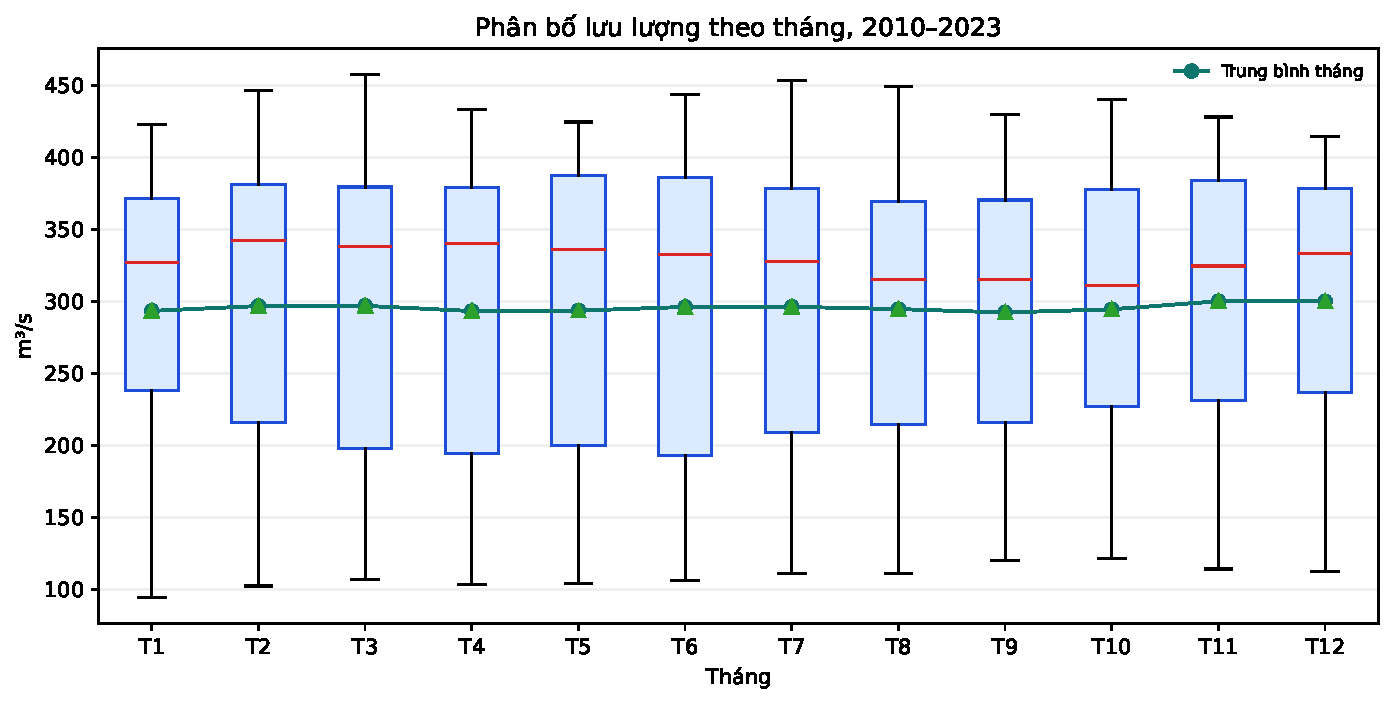
\includegraphics[width=0.93\linewidth]{monthly_boxplot.pdf}
\caption{Phân bố lưu lượng theo tháng. Các hộp chồng lấn mạnh, cho thấy mùa vụ theo
tháng yếu so với biến động giữa các năm.}
\label{fig:monthly-boxplot}
\end{figure}

Hình~\ref{fig:monthly-boxplot} cho thấy các hộp phân bố theo tháng chồng lấn gần như
hoàn toàn. Tháng 2 và tháng 3 có trung vị cao hơn, tháng 9 và tháng 10 có trung vị
thấp hơn, nhưng khoảng tứ phân vị rộng và nhiều giá trị ngoại lai ở cả hai phía.
Vì vậy không thể kết luận “mùa lũ” chỉ bằng tháng; cần xem thêm mức nền theo năm và
các đợt lưu lượng cao kéo dài.

\subsection{Xu hướng và sự thay đổi mức nền theo năm}

Bảng~\ref{tab:yearly-stats} (phụ lục) và Hình~\ref{fig:yearly-flow} cho thấy chuỗi
không có một xu hướng tuyến tính đơn giản. Giai đoạn 2010--2012 có mức nền thấp, với
trung bình năm 2010 chỉ \YearlyMinValue{} m\textsuperscript{3}/s. Từ 2013 đến 2020,
mức nền tăng rõ rệt; năm 2017 đạt trung bình \YearlyMaxValue{}
m\textsuperscript{3}/s, cao nhất trong 14 năm. Sau 2020, lưu lượng giảm dần: trung
bình năm 2021 là 305,25, năm 2022 là 231,00 và năm 2023 là 213,61
m\textsuperscript{3}/s. Biên độ trung bình giữa các năm lên tới \YearlyAmplitude{}
m\textsuperscript{3}/s, gấp khoảng 36 lần biên độ trung bình theo tháng.

\begin{figure}[H]
\centering
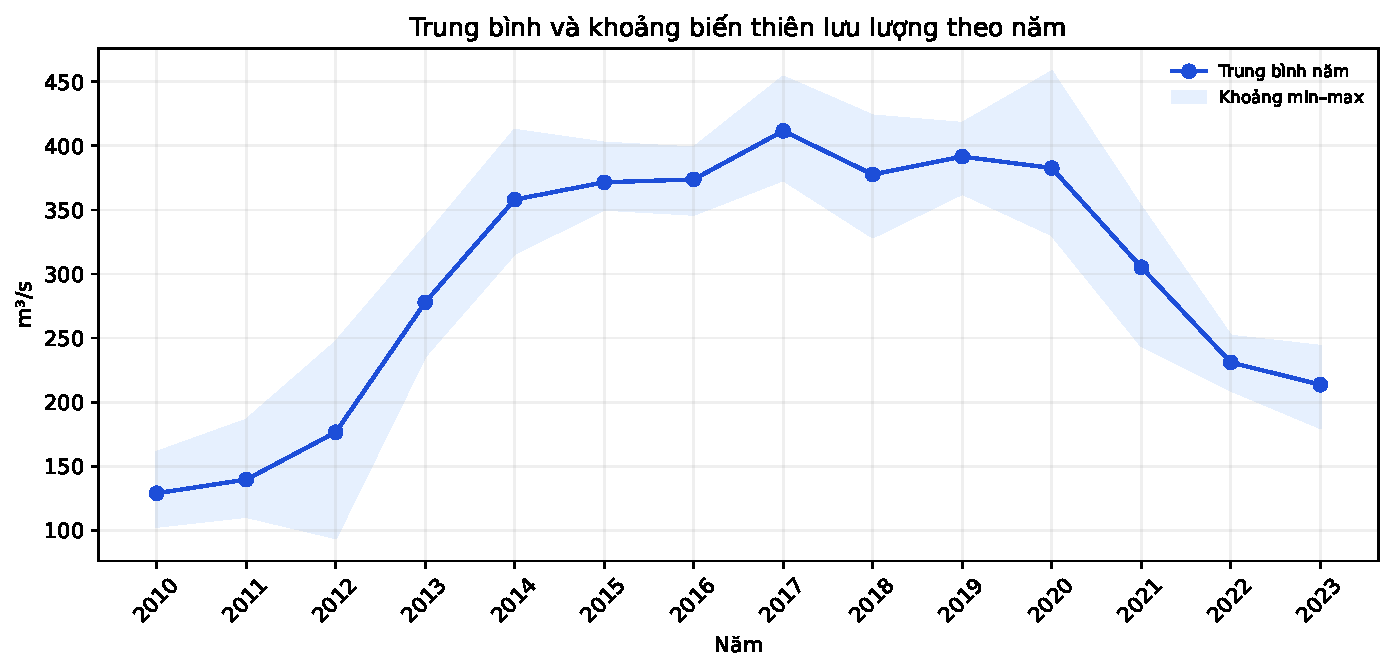
\includegraphics[width=0.95\linewidth]{yearly_flow.pdf}
\caption{Diễn biến lưu lượng ngày và trung bình trượt theo năm. Chuỗi có các giai
đoạn mức nền thấp, cao và suy giảm rõ rệt.}
\label{fig:yearly-flow}
\end{figure}

Sự thay đổi mức nền này quan trọng hơn mùa vụ theo tháng. Nếu chỉ nhìn trung bình
tháng, ta có thể kết luận chuỗi gần như phẳng; nhưng khi nhìn theo năm, ta thấy các
khối nhiều năm với mức lưu lượng rất khác nhau. Đây là lý do chính khiến mô hình
Seasonal Naive 365 hoạt động kém trên Test: nó lấy giá trị của cùng ngày năm trước,
trong khi mức nền giữa các năm đã thay đổi đáng kể.

\subsection{Phân rã STL}

Phân rã STL \cite{cleveland1990} với chu kỳ 365 ngày và tùy chọn robust được dùng
để tách chuỗi thành thành phần xu hướng, mùa vụ và phần dư. Kết quả cho thấy thành phần xu hướng chiếm
ưu thế: độ mạnh xu hướng là \TrendStrength{}, trong khi độ mạnh mùa vụ chỉ là
\SeasonalStrength{}. Hai giá trị này được tính từ tỷ lệ phương sai của thành phần
tương ứng sau khi loại bỏ phần dư; giá trị càng gần 1 thì thành phần đó càng quan
trọng.

\begin{figure}[H]
\centering
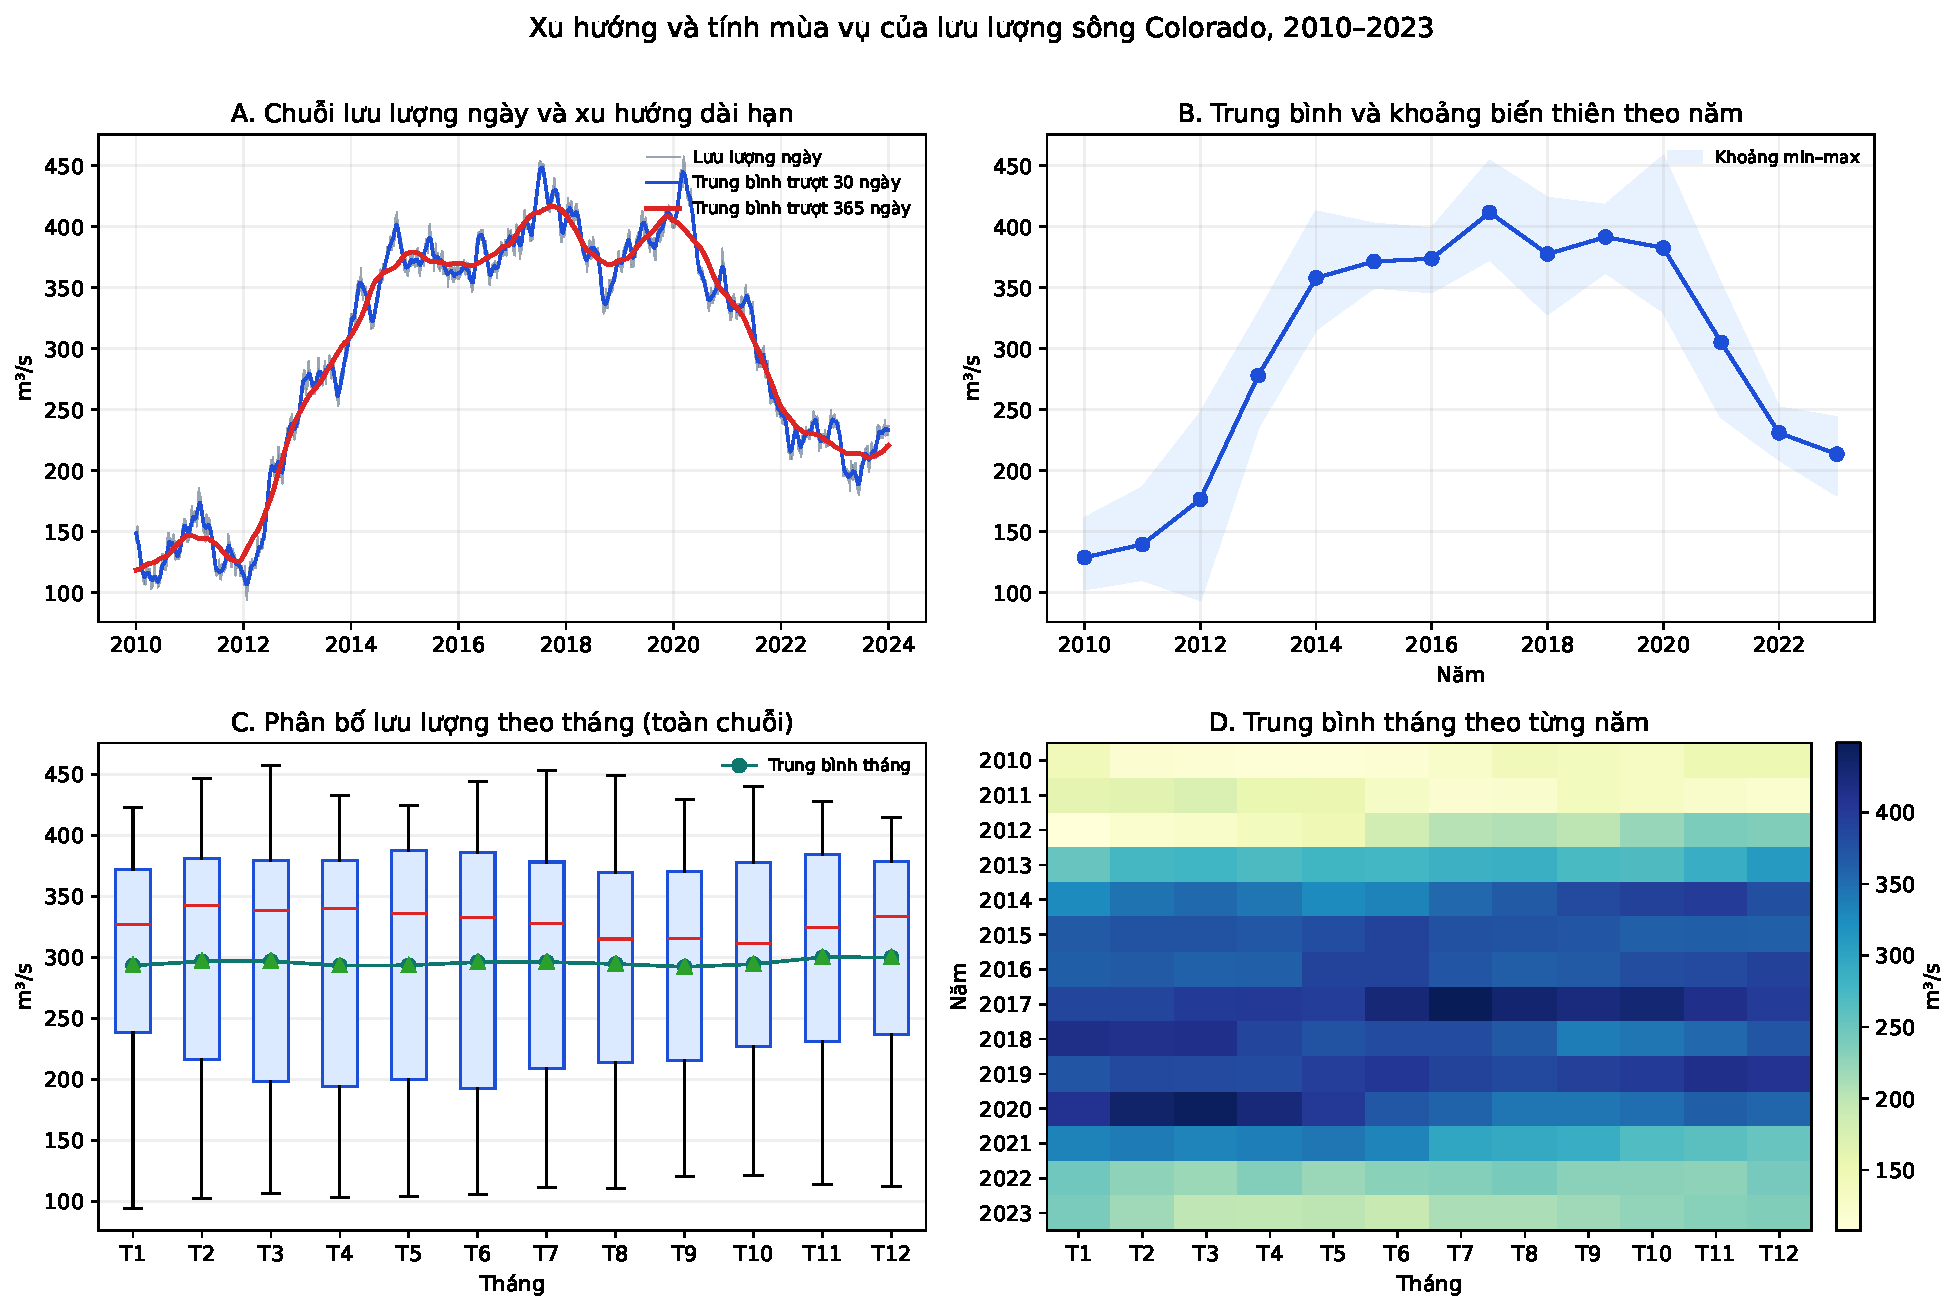
\includegraphics[width=0.95\linewidth]{trend_seasonality.pdf}
\caption{Bốn góc nhìn về xu hướng và mùa vụ: (A) chuỗi ngày và xu hướng dài hạn; (B) trung bình và khoảng biến thiên theo năm; (C) phân bố theo tháng; (D) trung bình theo năm và tháng.}
\label{fig:trend-seasonality}
\end{figure}

Thành phần xu hướng bắt đầu ở \TrendStart{} m\textsuperscript{3}/s, đạt cực đại
\TrendMax{} m\textsuperscript{3}/s và kết thúc ở \TrendEnd{}
m\textsuperscript{3}/s. Đây không phải là một đường thẳng tăng đều mà là một đường
cong mô tả sự chuyển đổi giữa các chế độ: thấp vào đầu giai đoạn, cao ở giữa và
giảm về cuối. Thành phần mùa vụ có biên độ nhỏ, dao động quanh mức vài
m\textsuperscript{3}/s; phần dư vẫn còn biến động đáng kể, phản ánh các sự kiện ngắn
hạn và các yếu tố chưa được mô hình hóa.

\begin{figure}[H]
\centering
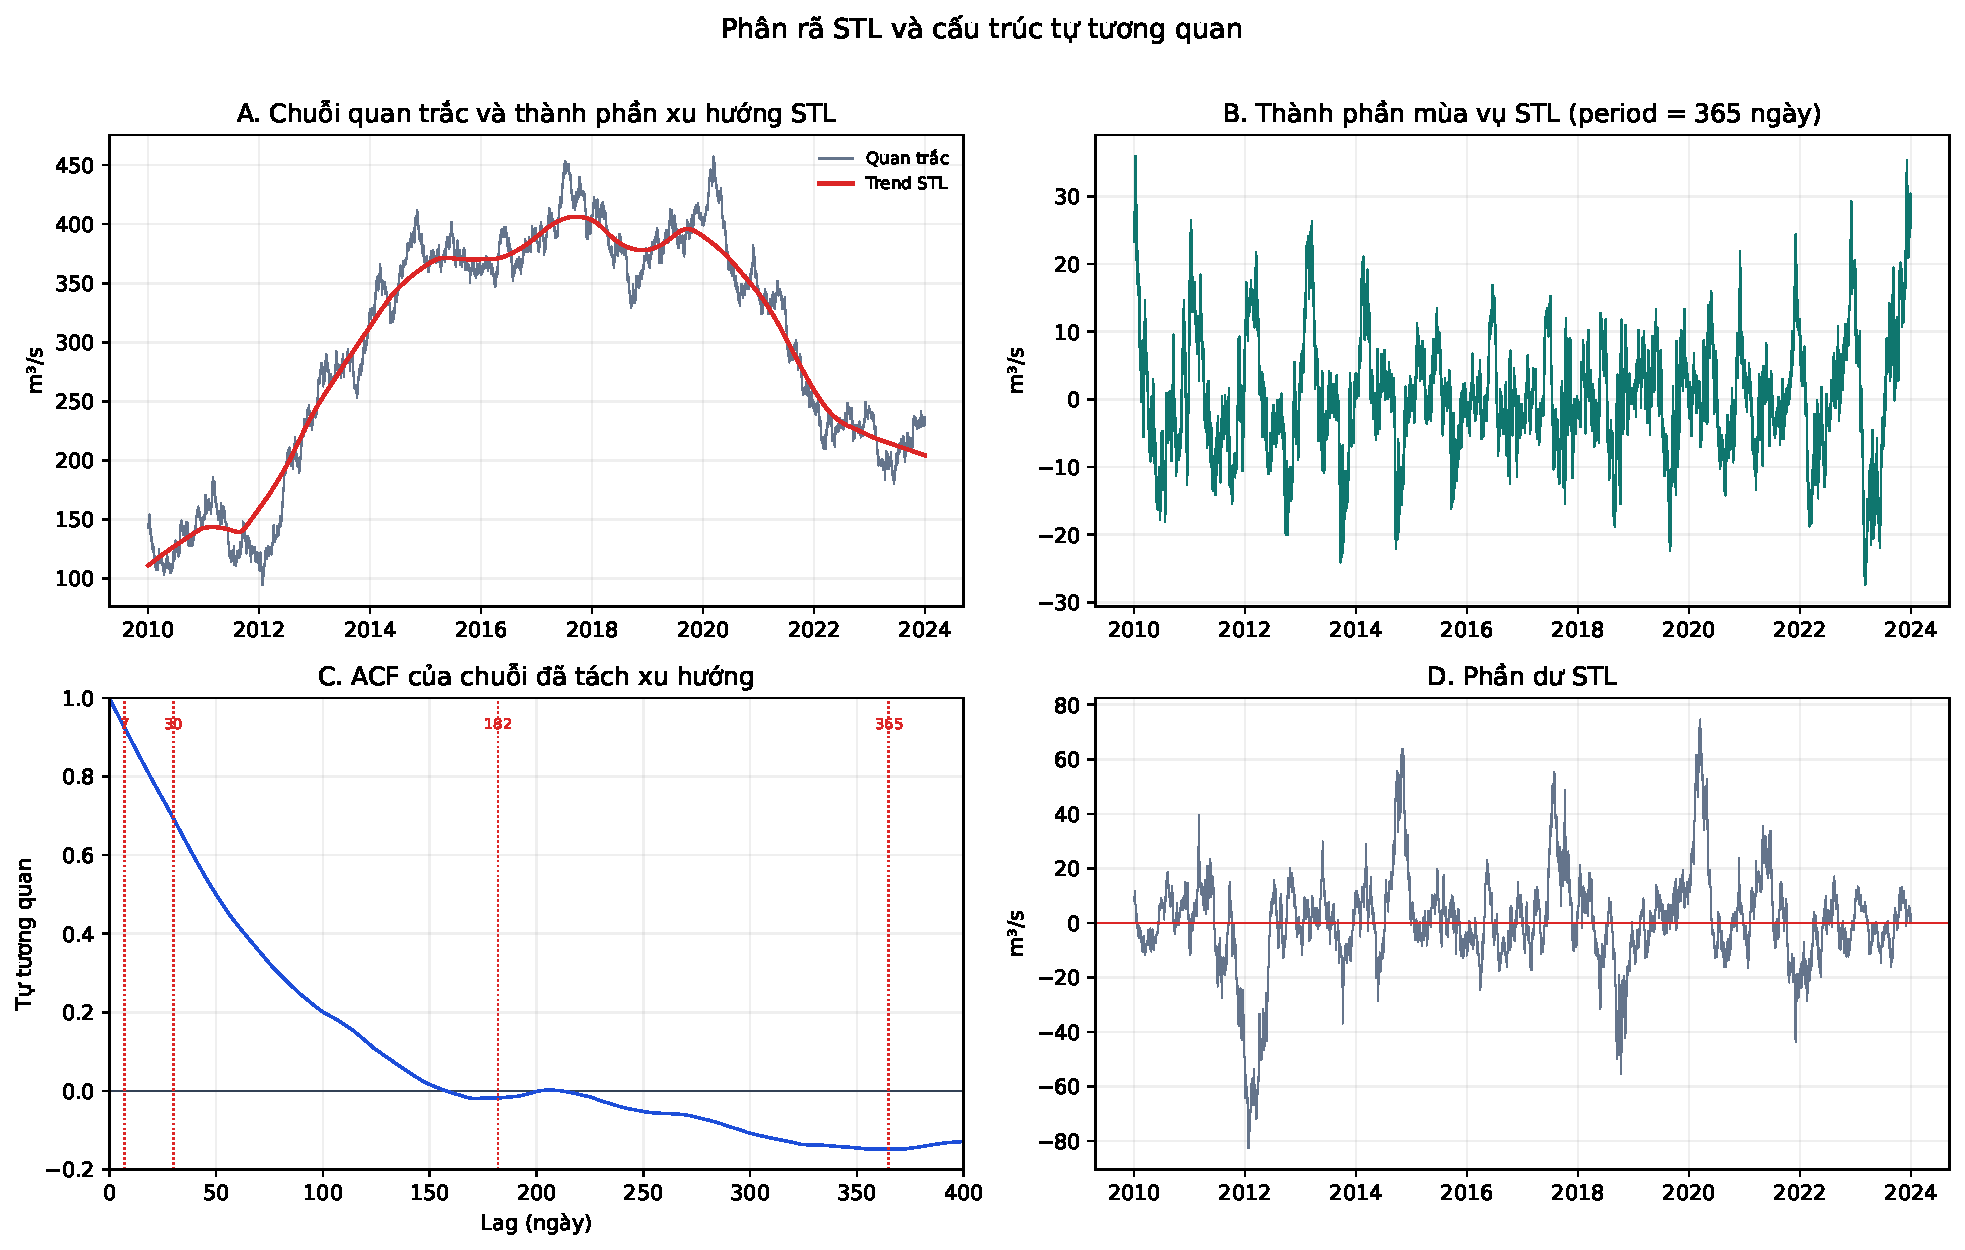
\includegraphics[width=0.92\linewidth]{stl_seasonality.pdf}
\caption{Phân rã STL: (A) chuỗi quan trắc và thành phần xu hướng; (B) thành phần mùa vụ; (C) ACF của chuỗi đã loại xu hướng; (D) phần dư.}
\label{fig:stl-seasonality}
\end{figure}

\subsection{Cấu trúc tự tương quan}

Hàm tự tương quan của chuỗi mức cho thấy tính dai dẳng rất mạnh ở các độ trễ ngắn:
ACF bậc 7 là \AcfSeven{}, bậc 30 là \AcfThirty{}. Tương quan giảm dần nhưng vẫn còn cao ở
các độ trễ hàng tháng. Ở độ trễ nửa năm, ACF gần bằng không (\AcfOneEightyTwo{}); ở độ trễ
một năm, ACF âm nhẹ (\AcfYear{}). Kết quả này cho thấy chuỗi không lặp lại ổn định
theo chu kỳ 365 ngày; mùa vụ theo năm không đủ mạnh để tạo tương quan dương ở độ trễ
một năm.

ACF giảm chậm là dấu hiệu của chuỗi có mức nền thay đổi hoặc gần với một quá trình
có nghiệm đơn vị. Báo cáo không chạy kiểm định ADF/KPSS vì mục tiêu chính là mô tả
và dự báo thực nghiệm, nhưng cấu trúc ACF đủ để giải thích vì sao mô hình Naive lại
là một baseline mạnh. Giá trị hôm nay chứa rất nhiều thông tin về ngày mai; các mô
hình phức tạp chỉ có thể cải thiện nếu chúng học được phần thay đổi nhỏ vượt trên
tính dai dẳng đó.

\subsection{Trả lời câu hỏi 1}

Từ các phân tích trên, có thể kết luận:

\begin{itemize}[leftmargin=1.4em]
  \item Chuỗi có xu hướng dài hạn dạng chuyển đổi chế độ, không tuyến tính; mức nền
  tăng từ 2010 đến khoảng 2017--2020 rồi giảm trong 2021--2023.
  \item Mùa vụ theo tháng tồn tại nhưng yếu: biên độ trung bình theo tháng chỉ
  \MonthlyAmplitude{} m\textsuperscript{3}/s, trong khi biên độ theo năm là
  \YearlyAmplitude{} m\textsuperscript{3}/s.
  \item Tính dai dẳng ngắn hạn rất mạnh: ACF bậc 7 là \AcfSeven{} và bậc 30 là
  \AcfThirty{}; tương quan ở độ trễ một năm âm nhẹ.
  \item Vì mùa vụ yếu và mức nền thay đổi, các mô hình dựa trên “cùng ngày năm
  trước” có nguy cơ sai lệch lớn; các mô hình dùng lag gần và rolling window là
  lựa chọn hợp lý về mặt cấu trúc, dù kết quả thực nghiệm cho thấy lợi ích so với
  Naive là rất nhỏ.
\end{itemize}

Những kết luận này định hướng cho phần dự báo: cần giữ Naive làm baseline, dùng
LightGBM với đặc trưng lag/rolling và mục tiêu delta, đồng thời đánh giá riêng từng
horizon thay vì chỉ nhìn một chỉ số trung bình.
